\chapter{Schlussbetrachtung}
\label{cha:schlussbetrachtung}

Im folgenden Kapitel wird die gesamte Arbeit rekapituliert. Dabei wird anhand der Vorgehensweise nochmals auf die wichtigsten Erkenntnisse eingegangen und diese erläutert. Anhand eines kurzen Ausblicks werden Anregungen für weitere Untersuchungen gegeben.

\section{Fazit}
\label{sec:fazit}

Gegenstand der Arbeit war die Konzeptionierung und Implementierung einer Android Applikation zur Raumbuchung via \acl{CUI}. Dazu wurden zunächst die Anforderungen an ein \ac{CUI} im Allgemeinen und auch im Kontext der Raumbuchung mit Hilfe von Methoden aus dem Bereich Usability Engineering betrachtet. 

In diesem Zusammenhang konnten mit Hilfe eines Fragebogens, Interviews und der Entwicklung von Personae ausführliche Einblicke in das Buchungsverhalten der Nutzer gewonnen werden. Hierbei wurde klar, dass die Ziele und Absichten der User sehr kontextspezifisch sind. So hat beispielsweise ein Mitarbeiter aus dem Bereich \textit{Human Resources} ein ganz anderes Verhalten und Präferenzen bei der Buchung als jemand aus dem Bereich \textit{Coaching}. Schnell wurde deutlich, dass diese Unterschiede erkannt und verinnerlicht werden müssen, bevor ein sinnvolles und zielgerichtetes Protoyping überhaupt stattfinden kann. 

Anhand von Papier-Prototypen und deren anschließender Umsetzung anhand eines Klickdummys konnten die ersten Ansätze auf ihre Plausibilität hin untersucht werden, bevor sie dann im Prototyping Tool umgesetzt wurden. Diese verschiedenen Ebenen des Prototypings sind eine gute Hilfe, um am Anfang uneingeschränkt und kreativ Ideen aufbringen zu können, diese anschließend möglichst schnell einem \textit{plausibility check} zu unterziehen und abschließend zu entscheiden, ob diese weiterverfolgt oder verworfen werden. 

Anschließend stand der Workflow, also die Vorgehensweise vom Anfang bis zum Abschluss der Buchung, im Vordergrund. Hierfür wurden auf Grundlage der Ergebnisse aus dem Requirements Engineering und in Anlehnung an die entwickelten Personae verschiedene Szenarien entworfen. Für jedes Szenario wurden dabei die unterschiedlichen Möglichkeiten und Wege bis zum Ende der Buchung betrachtet und anhand von Entscheidungsbäumen dargestellt. Dabei wurde deutlich, dass es je nach Art des Szenarios große Unterschiede in Bezug auf die Variation der Nutzeranfrage gibt. Im Kapitel \ref{subsec:workflow} wurde dabei zum einfacheren Verständnis das weniger umfangreiche Szenario aus dem Bereich \textit{Vertrieb} gewählt. Für ein anderes Szenario steigt der Umfang der möglichen Eingangsformulierungen des Users allerdings schnell auf bis zu zwölf Zweige an. Dies verdeutlicht die enorme Variabilität des Nutzers bei der Verwendung eines \aclp{CUI}.

Durch die Umsetzung der Ansätze mit Hilfe des Prototyping Tools werden schnell Probleme beim Workflow oder im mentalen Modell des Nutzers erkannt. Der Vorteil ist hierbei, dass diese Probleme noch im Status der Konzeption bzw. im Prototyping behoben werden können. In Abbildung \ref{fig:kosten-fehlerbehebung-softwareentwicklung} sind die Kosten der Fehlerbehebungen in der Softwareentwicklung über die verschiedenen Entwicklungsphasen dargestellt. Die Vorgehensweise nach dem Motto \textit{„test early - fail early“} spart hierbei also sowohl Zeit und Aufwand, als auch Kosten.
\newline
\begin{figure}[H]
    \centering
    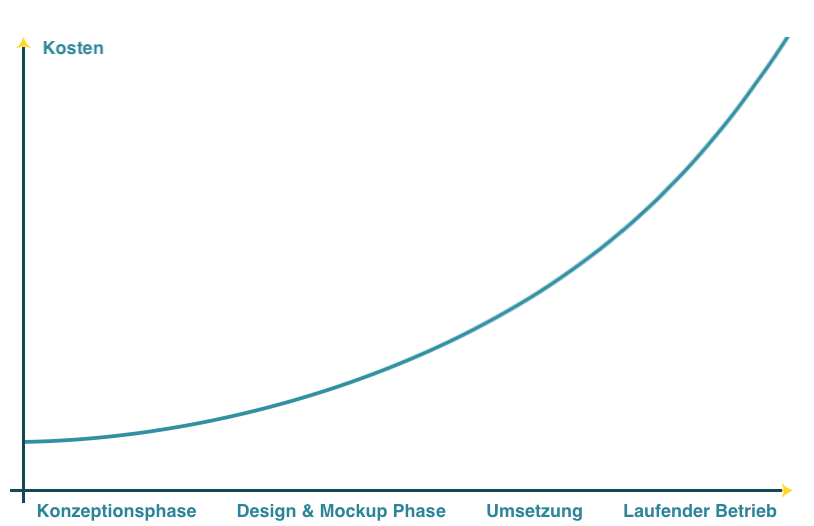
\includegraphics[width=0.9\textwidth]{bilder/fehlerkostensoftware.png}
    \caption{Kosten der Fehlerbehebung in der Softwareentwicklung \cite{claus_degendorfer_wie_2016}}
    \label{fig:kosten-fehlerbehebung-softwareentwicklung}
\end{figure}

Die prinzipielle Idee eines \acl{CUI} mit der Kombination aus Text und \ac{UI}-Elementen im Kontext einer Raumbuchung ist für die Nutzer verständlich. Dies bestätigen die Ergebnisse und Rückmeldungen aus den User Tests. Zudem bieten diese gute Ansatzpunkte für eine weitere Bearbeitung der Thematik. Darauf soll explizit noch im Folgekapitel \textit{\nameref{sec:ausblick}} eingegangen werden.

Wie auch dem Umfang der entsprechenden Kapitel \textit{\nameref{cha:konzeption}} und \textit{\nameref{cha:implementierung}} zu entnehmen ist, stellt die konzeptionelle Betrachtung einen großen Teil der Arbeit dar. Wie zuvor erläutert ist dies gleichermaßen wichtig wie notwendig, um ein fundiertes Verständnis über die Thematik zu erhalten. Nichtsdestotrotz ist auch die Implementierung ein fester Bestandteil der Arbeit und wurde entsprechend umgesetzt. Durch die Auswahl der Komponenten und deren Aufbau sowie die Klärung ihrer Kommunikation und Schnittstellen konnte hierbei ein solides Grundgerüst für eine weitere Implementierung aufgebaut werden. Einige der im Prototyping erprobten Ansätze in Bezug auf den Konversationsfluss und der \ac{UI}-Elemente konnten hierbei bereits einfließen. Dem Nutzer ist es möglich, mit Hilfe der Android Applikation nach freien Räumen im Office der \adorsys\ zu suchen und einen Besprechungsraum zu reservieren.

\section{Ausblick}
\label{sec:ausblick}
Aufgrund des begrenzten Zeitrahmens in Abschlussarbeiten können meist leider nicht alle Inhalte einer Thematik ausreichend beleuchtet oder umgesetzt werden. Daher dient dieses Unterkapitel dazu, einige Anmerkungen und Ausblicke für weitere Betrachtungen aufzugreifen und zu erläutern. 

Wie bereits eingangs erwähnt, dient Sprache sowohl der schriftlichen als auch der mündlichen Konversation. In dieser Arbeit lag der Fokus auf der Entwicklung eines textuellen \acp{CUI} in Form eines Chatbots. Denkbar wäre hier also eine Erweiterung des Systems um eine sprachbasierte Eingabemöglichkeit. Dabei wird die gesprochene Sprache über ein Mikrofon aufgenommen und über \textit{\ac{ASR}} in Textform konvertiert. Die textuelle Sprache kann anschließend weiter verarbeitet werden. Der Rückweg zur Ausgabe des Audiosignals wird dann mit Hilfe von \textit{\ac{TTS}} realisiert.

Während der Durchführung der User Tests kam häufig die Frage nach einem Namen oder dem Aussehen des Chatbots auf. Viele Nutzer haben einen Charakter des Chatbots erwartet oder gar vermisst. In diesem Zusammenhang erscheint ein Charakterdesign für den Chatbot als sinnvoll. Dabei erhält der Chatbot einen Namen und einen Avatar, was ihn für den User transparenter und sympathischer macht. 

Nahezu unverzichtbar ist für den Kontext einer Raumbuchung natürlich die Einladung von weiteren Personen. Dieser Teil wurde im Rahmen der Arbeit bewusst zunächst außen vor gelassen, muss aber früher oder später fester Bestandteil des Systems sein. Großen Mehrwert hat das System hier bei der Terminfindung. So können beispielweise alle Teilnehmer eines Meetings angegeben und der nächstmögliche freie Termin inklusive passendem Raum vorgeschlagen werden. Eine ergänzende Idee ist hierbei, im System gewisse Teams zu hinterlegen. So könnte der User beispielsweise nur angeben, er möchte alle Mitglieder aus dem \textit{iOS-Team} zu einem Termin einladen und das System schlägt ihm mögliche Zeiträume vor, bei dem alle oder zumindest ein Großteil der Teilnehmer verfügbar ist. 

Enormes Potenzial für den Anwendungsfall der Raumbuchung bietet auch die Technologie des \aclp{ML}. Bis zum derzeitigen Stand der Arbeit befindet sich \acl{ML} nur im Bereich der \ac{NLP}-Plattform. Dies passiert jedoch unter der Oberfläche von Dialogflow und stellt somit keinen direkten Berührungspunkt dar. Eine eigene Umsetzung aus dem Bereich \ac{ML} im Rahmen des \aclp{DM} könnte die Intelligenz des Systems wesentlich verbessern. Ein mögliches Anwendungsgebiet ist hierbei das Erkennen und Erlernen von Verhaltensmustern eines Nutzers bei der Buchung. Damit wäre das System in der Lage, für einen Nutzer spezifische Vorhersagen über die Raumpräferenzen oder die Auswahl von Vor- und Nachbereitungszeit für einen Termin zu treffen. 